% One run of a compiled function that draws three times from the global random
% state: R hands the key and the counter to the program as implicit inputs,
% every draw splits at its own counter, computed from the one the program took,
% and after the run R advances the counter by the number of draws, which was
% known when the function was traced. The program returns no random state.
% Build: see figures/README.md
\documentclass[tikz, border = 6pt]{standalone}
\usepackage[T1]{fontenc}
\usepackage{lmodern}
\usepackage{amsmath}
\usetikzlibrary{positioning, calc, arrows.meta, fit, backgrounds}

\definecolor{hash}{HTML}{5B8C5A}
\definecolor{keep}{HTML}{2A7AB0}
\definecolor{fork}{HTML}{E08A2C}

\tikzset{
  >={Stealth[length = 2mm]},
  lane/.style = {draw = black!25, fill = black!3, rounded corners = 4pt},
  lanetitle/.style = {font = \small\bfseries, text = black!70, anchor = north west},
  state/.style = {draw, rounded corners = 2pt, inner sep = 4pt, align = center,
    font = \small},
  input/.style = {draw = keep!80!black, fill = keep!15, rounded corners = 2pt,
    inner sep = 3pt, font = \ttfamily\small, minimum height = 6mm},
  call/.style = {draw = hash!80!black, fill = hash!15, rounded corners = 2pt,
    inner sep = 3pt, font = \ttfamily\footnotesize, minimum height = 6mm,
    align = left},
  counter/.style = {draw = black!50, fill = white, rounded corners = 2pt,
    inner sep = 3pt, font = \ttfamily\footnotesize, minimum height = 6mm},
  note/.style = {font = \footnotesize, text = black!65, align = left},
  edge/.style = {->, black!70},
  flow/.style = {->, very thick, black!55},
  elabel/.style = {font = \footnotesize, fill = white, inner sep = 1pt}
}

\begin{document}
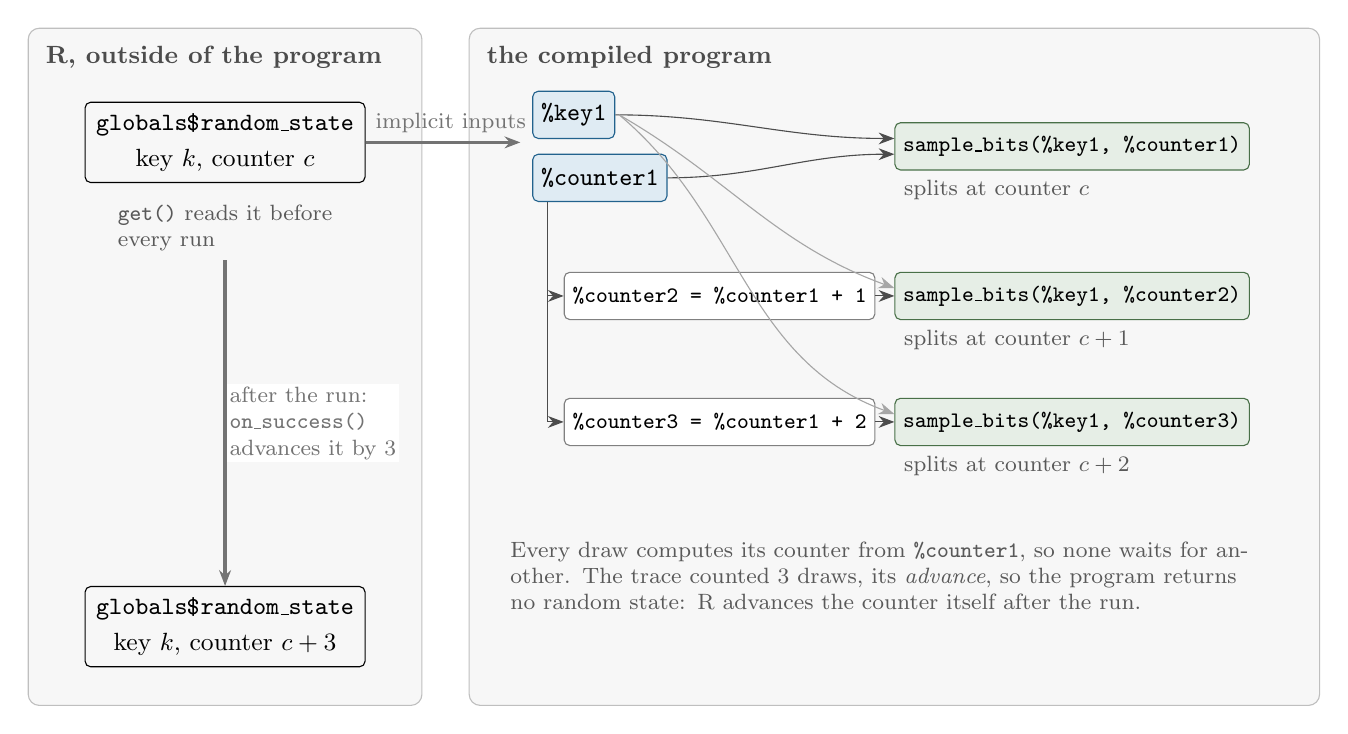
\begin{tikzpicture}

  % ---- lanes -------------------------------------------------------------
  \fill[black!3, draw = black!25, rounded corners = 4pt] (-0.4, 1.0) rectangle (4.6, -7.6);
  \node[lanetitle] at (-0.3, 0.9) {R, outside of the program};
  \fill[black!3, draw = black!25, rounded corners = 4pt] (5.2, 1.0) rectangle (16.0, -7.6);
  \node[lanetitle] at (5.3, 0.9) {the compiled program};

  % ---- before the run ----------------------------------------------------
  \node[state] (before) at (2.1, -0.45)
    {\texttt{globals\$random\_state}\\[2pt]key $k$, counter $c$};

  % ---- the program's inputs ----------------------------------------------
  \node[input, anchor = west] (key) at (6.0, -0.1) {\%key1};
  \node[input, anchor = west] (counter) at (6.0, -0.9) {\%counter1};
  \draw[flow] (before.east) -- node[elabel, above = 2pt, pos = 0.55, fill = none] {implicit inputs}
    (5.85, -0.45);

  % ---- three draws, each at its own counter ------------------------------
  \node[call, anchor = west] (d1) at (10.6, -0.5)
    {sample\_bits(\%key1, \%counter1)};
  \node[counter, anchor = west] (c2) at (6.4, -2.4) {\%counter2 = \%counter1 + 1};
  \node[call, anchor = west] (d2) at (10.6, -2.4)
    {sample\_bits(\%key1, \%counter2)};
  \node[counter, anchor = west] (c3) at (6.4, -4.0) {\%counter3 = \%counter1 + 2};
  \node[call, anchor = west] (d3) at (10.6, -4.0)
    {sample\_bits(\%key1, \%counter3)};

  \draw[edge] (key.east) to[out = 0, in = 180] ($(d1.west) + (0, 0.1)$);
  \draw[edge] (counter.east) to[out = 0, in = 180] ($(d1.west) + (0, -0.1)$);
  \draw[edge] ($(counter.south west) + (0.2, 0)$) |- (c2.west);
  \draw[edge] ($(counter.south west) + (0.2, 0)$) |- (c3.west);
  \draw[edge] (c2) -- (d2);
  \draw[edge] (c3) -- (d3);
  \draw[edge, black!35] (key.east) ++(0.05, 0) to[out = -30, in = 160] ($(d2.west) + (0, 0.1)$);
  \draw[edge, black!35] (key.east) ++(0.05, 0) to[out = -40, in = 160] ($(d3.west) + (0, 0.1)$);

  \node[note, anchor = north west] at (d1.south west) {splits at counter $c$};
  \node[note, anchor = north west] at (d2.south west) {splits at counter $c + 1$};
  \node[note, anchor = north west] at (d3.south west) {splits at counter $c + 2$};

  \node[note, anchor = north west, text width = 9.6cm] at (5.6, -5.4)
    {Every draw computes its counter from \texttt{\%counter1}, so none waits for
     another. The trace counted 3 draws, its \emph{advance}, so the program
     returns no random state: R advances the counter itself after the run.};

  % ---- after the run -----------------------------------------------------
  \node[note, below = 0.15 of before] (read) {\texttt{get()} reads it before\\every run};
  \node[state] (after) at (2.1, -6.6)
    {\texttt{globals\$random\_state}\\[2pt]key $k$, counter $c + 3$};
  \draw[flow] (read.south) -- node[elabel, right, align = left, pos = 0.5]
    {after the run:\\\texttt{on\_success()}\\advances it by 3} (after.north);

\end{tikzpicture}
\end{document}
